\graphicspath{{testing_and_validation/fig/}}

\chapter{Testing \& Validation}

The testing and validation process was structured to systematically verify the functionality of the impedance analyser, progressing from subsystem verification to complete system integration and finally calibration and validation with actual biosensors. This methodical approach allowed for the identification and correction of issues at each stage, ensuring that problems could be isolated and resolved before integration with more complex subsystems.

% Testing began with fundamental verification of the assembled PCB, followed by individual subsystem characterisation. Once subsystem functionality was established, the complete analogue frontend was tested as an integrated system. Finally, the device was calibrated against the PalmSens4 impedance analyser and validated using biosensors with buffer solutions.

\section{PCB Testing}

Upon receiving the assembled PCB visual inspection and continuity testing confirmed no obvious short circuits or discontinuities. The ESP32's onboard battery charging circuit was confirmed to supply a stable 3.3 V rail to all digital and analogue components. The virtual ground reference circuit was measured at exactly 1.650 V. The TPS61072 boost converter successfully provided a stable 5 V supply for the LTC1069 anti-aliasing filter.

Next, each subsystem was tested individually whilst other subsystems remained disconnected. This approach allowed for precise characterisation of each stage's performance and simplified fault diagnosis.

\subsection{Excitation Stage} 
The excitation stage was tested using a signal generator providing a 3 Vpp input signal and an oscilloscope to measure the attenuated output. Unfortunately, the LTC1069 anti-aliasing filter was found to be dead-on-arrival. Given the significant lead times for component procurement and project time constraints, it was not feasible to order a replacement. The filter was therefore bypassed, and the excitation stage was tested without it. Whilst this introduces higher-frequency components from the DAC's stairstepping, the synchronisation of DAC generation and ADC sampling in the final system helps to minimise the impact on measurements.

The attenuation stage was characterised across the full frequency range from 1 Hz to 100 kHz. The resulting signal was measured at ~10.33 mV, giving a 290 V/V attenuation. This is close to the designed 300 V/V with the variation likely due to component tolerances.

% Figure \ref{fig:excitation_freq_response} shows the frequency response, which exhibits a flat gain and phase across the measurement range.
% Move fig to appendix
% \begin{figure}[H]
%     \centering
%     % \includegraphics[width=0.8\textwidth]{ExcitationFreqResponse.png}
%     \caption{Excitation Stage Frequency Response}
%     \label{fig:excitation_freq_response}
% \end{figure}

\subsection{Voltage Measurement Stage} 
For the voltage measurement stage, both the INA331 instrumentation amplifier and TLV9061 gain stage were tested separately. The INA331 was tested using a 200mV input signal to minimise noise. It performed as expected, with no measurable gain roll-off at 100 kHz and a phase shift of -5\textdegree, which is close to the expected -4.6\textdegree based on simulations.

Initial testing of the TLV9061 stage showed a completely unstable system. Investigation uncovered a critical oversight in the PCB design. The TLV9061 op-amp symbol used in KiCad had a different pinout than the LTspice model used for simulation, resulting in the inverting and non-inverting inputs being swapped. This was corrected through careful trace cutting and wire jumpers, and the corrected schematic was updated in KiCad for future PCB revisions. After this modification, the TLV9061 stage performed well, exhibiting a -8.7° phase shift at 100 kHz compared to the expected -3.4°. The larger-than-expected phase shift can be attributed to several factors including the additional parasitic capacitance introduced by the rework, tolerances in the op-amp's gain-bandwidth product, and PCB layout effects not fully captured in simulation. The measured gain roll-off at 100 kHz was less than 0.2 dB. 

Overall, the voltage measurement stage's performance closely matched expectations, with the phase discrepancies remaining well within acceptable limits for accurate impedance measurements if properly calibrated for.

\todo{Insert Table wat cutoff en 100kHz summarise vir elke afdeling en dan langs dit grafiek wat responses van elke substage wyse op eenm grafiek}


\subsection{Current Measurement Stage} 
The current measurement stage required the most extensive testing due to its complexity and switchable gain configurations. Significant concerns existed regarding the TIA functionality given the extremely small 0.4 mm pitch BGA package of the OPA3S328, however testing confirmed it operated correctly.

The TIA was characterised by applying known voltages across resistors of known values, allowing the input current to be calculated. The TIA output voltage was then measured to determine the transimpedance gain across the full frequency range. Whilst the resistor values were measured using a standard multimeter (rather than a kelvin sens connection) and the resistor's parasitic inductance and capacitance was ignored, this characterisation served primarily for functional validation, as final calibration would be performed against the PalmSens4. 

At $R_f = 37.5\,\Omega$, the TIA exhibited a gain of 37.73 V/V with a phase shift of -4.4\textdegree and gain reduction of 0.74 dB at 100 kHz. At the larger feedback resistor value of $R_f = 7.5\,k\Omega$, the gain averaged at 7427. Interestingly, both phase shift and gain reduction  at 100 kHz were less pronounced at -3.5\textdegree and \textless 0.1 dB respectively. This is possibly due to slight peaking.

Stability was verified by connecting a simplified Randles equivalent circuit with a constant capacitance of \SI{1.47}{\micro F} and resistance of $12 \Omega$, approximating the expected biosensor characteristics. A 10 mVpp signal was applied to the equivalent circuit and swept from 1 Hz to 30 MHz while monitoring the TIA output for oscillations, ringing, or excessive peaking in the frequency response. No instability was observed, confirming the theoretical analysis in Section \ref{subsec:design_cur}.

The PGA113 was measured at each gain setting from 1 V/V to 200 V/V for each measurement frequency. Table \ref{tab:pga_performance} shows the measured gain and phase shift at 100 kHz for each setting. As expected, the phase shift is noticable at higher gain settings, however the higher gains will primarily be used at lower frequencies where the phase shift is negligible. These gain and phase shift values were incorporated into the calibration procedure to ensure accurate impedance calculations.

\begin{table}[H]
\centering
\caption{PGA113 Performance at 100 kHz}
\label{tab:pga_performance}
\begin{tabular}{|c|c|c|c|c|}
\hline
\textbf{Gain Setting} & \textbf{Max Gain} & \textbf{100kHz Gain} & \textbf{Gain Reduction} & \textbf{100kHz Phase} \\
\textbf{(V/V)} & \textbf{(V/V)} & \textbf{(V/V)} & \textbf{(dB)} & \textbf{Shift (\textdegree)} \\
\hline
1 & 1.00 & 0.92 & -0.74 & -0.8 \\
\hline
2 & 2.00 & 1.84 & -0.71 & -2.132 \\
\hline
5 & 4.98 & 4.57 & -0.74 & -1.634  \\
\hline
10 & 9.97 & 9.15 & -0.74 & -2.613 \\
\hline
20 & 21.60 & 21.52 & -0.03 & -5.619 \\
\hline
50 & 54.00 & 53.44 & -0.09 & -7.491 \\
\hline
100 & 99.92 & 92.18 & -0.70 & -14.79 \\
\hline
200 & 198.06 & 173.17 & -1.17 & -25.73 \\
\hline
\end{tabular}
\end{table}

The final TLV9061 amplification stage in the current measurement path was modified using the same trace cutting and rewiring procedure as the voltage measurement stage. Measurements confirmed no measurable difference in performance compared to the voltage measurement path, ensuring that gain reductions and phase shifts cancel out during impedance calculation as designed.

\section{System Calibration}

With all subsystems verified individually, the system was integrated and calibrated. The complete analogue frontend was tested using passive test cells, initially with a signal generator providing the excitation. Once analogue system stability and measurement accuracy were confirmed, the STM32 was used to generate DAC signals and acquire responses with the ADCs.

\trimdown{The STM32's ADC offsets were calibrated using the built-in functions. The gradients were determined by applying a series of known voltages using a bench power supply, with each voltage verified using an oscilloscope and multimeter. Similarly, the DAC output was measured, and the centre point of the generated signal adjusted from 2048 to 2009 to account for the constant voltage offset in the excitation stage attenuation. This ensured that the analogue output was precisely centred at 1.65 V, ensuring the biosensor is not biased with a DC voltage.The DAC's frequency generation capability was verified by measuring the output waveform at each test frequency using an oscilloscope. }
% Frequency was confirmed to be accurate across the entire range, validating the timer configuration and DMA-based waveform generation. 
% Initial calibration attempts using precision resistors measured with the PalmSens4 across the full frequency range (to account for parasitic impedances) proved problematic. Each TIA and PGA gain combination was calibrated separately using these measurements. However, when testing Randles equivalent circuits or actual biosensors, the frequency-dependent impedance characteristics resulted in unacceptably large error margins. \rephrase{The fixed PGA gain used during calibration did not match the actual measurement conditions, where gain settings vary with frequency to maintain optimal ADC range utilisation.}
% This necessitated a revised calibration approach. The gain settings for each frequency were pre-programmed to match the expected impedance range based on PalmSens4 characterisation of the biosensors. 
Frequency response data from each subsystem was smoothed with Locally Estimated Scatterplot Smoothing (LOESS) filtering in MATLAB to minimise measurement noise. The processed data was compiled into a calibration table. Finally, a non-faradaic Randles equivalent test cell (consisting of a 12 $\Omega$ resistor and 1.47 $\mu$F capacitor in series), was measured with both the BioPal and PalmSens4. This was used to calibrate the BioPal's response against the reference instrument. 
% This approach accounts for the complete signal chain at actual operating conditions, significantly improving accuracy.

It was found that at very low frequencies (32Hz and below), the lack of filtering in the excitation phase, lead to significant aliasing. Due to the \ac{DUT}'s lower impedance at higher frequencies, the aliased high-frequency components dominated the response, leading to clipping at high gain settings or conversely, very low signal levels at the frequency of interest for low gain settings. However, as shown in the following section, these frequencies are below the range of interest for the tested \acp{IDE} and thus did not have a significant impact on results. However, it did lead to increased error margins at lower frequencies, especially in phase measurements.

After calibrating the system, final validation could be done through measurements on \acp{IDE} using phosphate buffered saline (PBS) 1x solution and bovine serum albumin (BSA) protein.

\section{Final Validation}

Initial validation was performed using PBS 1x solutions of varying concentrations to test the BioPal's ability to measure bulk solution impedance changes. Following this, BSA protein binding to the \acp{IDE} was used to simulate antibody-antigen interactions, allowing validation of surface-based impedance changes.
% PBS 1× was selected as the electrolyte solution due to its physiological ionic strength and pH (7.4), which closely mimics the conditions in bodily fluids and provides a stable, well-characterised electrochemical environment for biosensor operation.
PBS solutions of v25\%, 50\% and 75\% concentrations were prepared by diluting stock PBS 1x with deionised water with higher PBS concentrations corresponding to higher ionic strength and thus lower solution impedance. Figures \ref{fig:25_pbs_comparison} - \ref{fig:75_pbs_comparison} show impedance measurements taken by both the BioPal and PalmSens4 for each concentration. Baseline measurements were taken using the diluted solutions, followed by final measurements using undiluted PBS 1x. Tabel \ref{tab:pbs} summarises the average reduction in impedance magnitude between the baseline and final measurements across the frequency range from 32 Hz - 100 kHz.

\begin{table}[H]
\centering
\caption{Average Impedance Change from Baseline to PBS 1x (32 Hz - 100 kHz)}
\label{tab:pbs}
\begin{tabular}{lcc}
\hline
\textbf{Concentration} & \textbf{PalmSens4 Reduction} & \textbf{BioPal Reduction} \\
\hline
% \hline
\textbf{25\%} & 45.3\% & 47.6\% \\
\textbf{50\%} & 33.8\% & 31.2\% \\
\textbf{75\%} & 12.9\% & 12.4\% \\
\hline
\end{tabular}
\end{table}
% The BioPal successfully detected the impedance increase following BSA adsorption, demonstrating its capability to measure surface-based electrochemical changes relevant to biosensing applications.

% PBS comparison figures
\begin{figure}[H]
    \centering
    \begin{subfigure}{0.48\textwidth}
        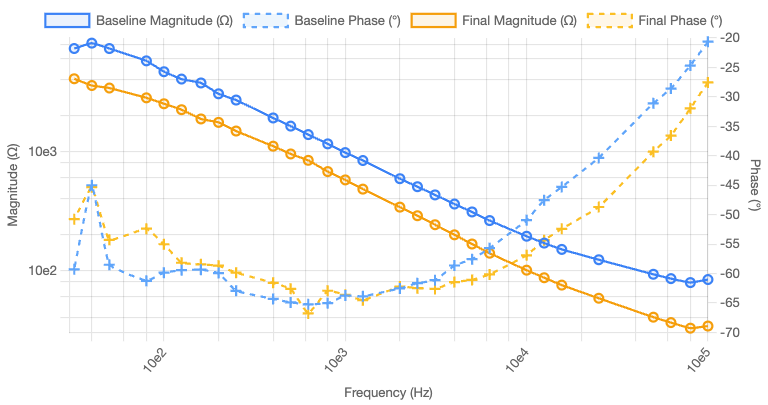
\includegraphics[width=\textwidth]{PBS_25_cropped.png}
        \caption{BioPal}
        \label{fig:25_pbs_biopal}
    \end{subfigure}
    \hfill
    \begin{subfigure}{0.48\textwidth}
        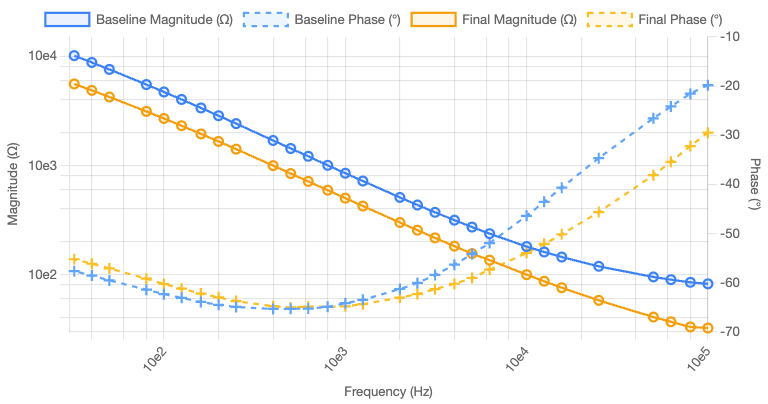
\includegraphics[width=\textwidth]{PalmSens_25.png}
        \caption{PalmSens4}
        \label{fig:25_pbs_palmsens}
    \end{subfigure}
    \caption{25\% Baseline vs 100\% Final PBS 1x Comparison}
    \label{fig:25_pbs_comparison}
\end{figure}

\begin{figure}[H]
    \centering
    \begin{subfigure}{0.48\textwidth}   
        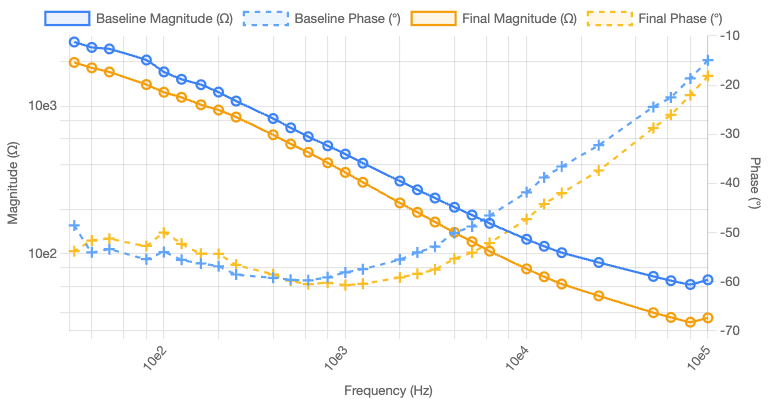
\includegraphics[width=\textwidth]{PBS_50_cropped.png}
        \caption{BioPal}
        \label{fig:50_pbs_biopal}
    \end{subfigure}
    \hfill
    \begin{subfigure}{0.48\textwidth}
        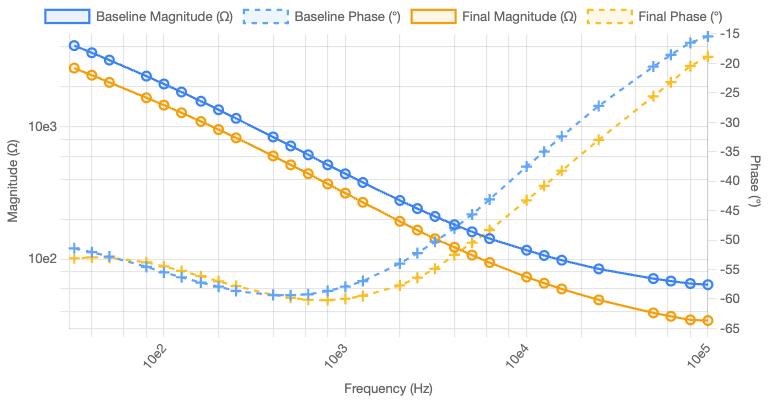
\includegraphics[width=\textwidth]{PalmSens_50.png}
        \caption{PalmSens4}
        \label{fig:50_pbs_palmsens}
    \end{subfigure}
    \caption{50\% Baseline vs 100\% Final PBS 1x Comparison}
    \label{fig:50_pbs_comparison}
\end{figure}

\begin{figure}[H]
    \centering
    \begin{subfigure}{0.48\textwidth}
        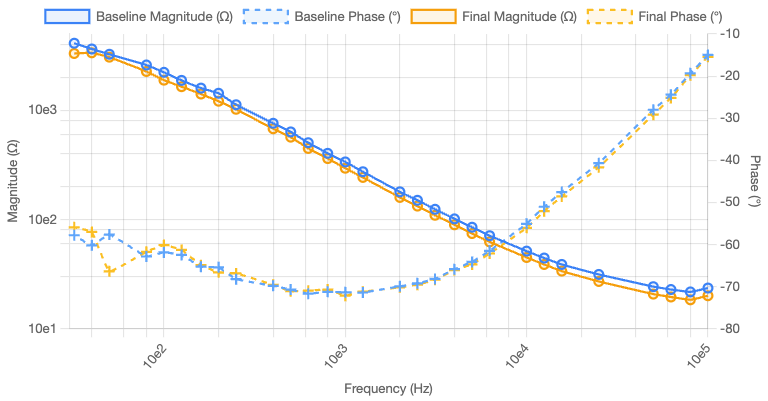
\includegraphics[width=\textwidth]{PBS_75_cropped.png}   
        \caption{BioPal}
        \label{fig:75_pbs_biopal}
    \end{subfigure}
    \hfill
    \begin{subfigure}{0.48\textwidth}
        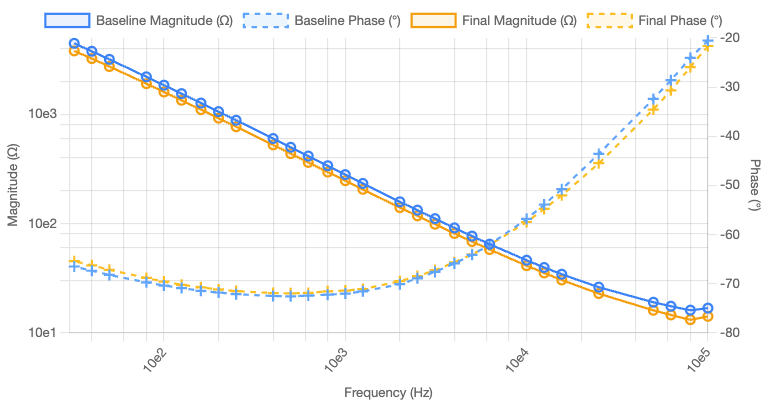
\includegraphics[width=\textwidth]{PalmSens_75.png}
        \caption{PalmSens4}
        \label{fig:75_pbs_palmsens}
    \end{subfigure}
    \caption{ 75\% Baseline vs 100\% Final PBS 1x Comparison}
    \label{fig:75_pbs_comparison}
\end{figure}

After validating the ability to distinguish bulk solution impedance changes, sensitivity to surface-based impedance changes needed to be confirmed. While testing with immobilised antibodies and actual protein antigens would provide the most direct validation, this was beyond the scope of this project due to laboratory safety restrictions, cost constraints, and limited time. Instead, BSA was used as a surface-binding protein to simulate antibody-antigen interactions. BSA is a common blocking protein that is readily absorbed by gold electrode surfaces, creating a protein layer that alters the interfacial impedance characteristics. This mimics the effect of antibody-antigen binding on the electrode surface.

The measurement methodology involved establishing a baseline impedance measurement in PBS 1x, removing the PBS and adding BSA solution to the electrode well, allowing 20 minutes for protein adsorption, flushing the electrode three times with fresh PBS 1x to remove unbound protein and thus maintaining the same solution characteristics, and finally performing a second impedance measurement.

Existing literature use BSA concentrations ranging from 1 mg/mL to 60 mg/mL for impedance based biosensor sensitivity validation \cite{maImpedancebasedIntegratedBiosensor2013}\cite{ebadiPolypyrrolebasedBovineSerum2025}. In this work, three concentrations were selected: 20 mg/mL, 50 mg/mL and 100 mg/mL.

Measurements were performed at each step using both the BioPal and the PalmSens4 for direct comparison. Figures \ref{fig:2g_bsa_comparison_final} - \ref{fig:10g_bsa_comparison_final} shows the impedance magnitude and phase measurements from both instruments before and after BSA binding, showing a clear difference between concentrations. Figures \ref{fig:2g_bsa_comparison} - \ref{fig:10g_bsa_comparison} show the relative change in magnitude across the frequency range. It was found that the largest impedance changes occurred in the frequency range from 160 Hz to 500 kHz. The average change in this range was used to give a qualitative result. The device gives the user a risk level of disease presence ranging from none to high based on the following thresholds:
\begin{table}[H]
\centering
\caption{Qualitative Risk Levels Based on Impedance Change}
\label{tab:risk_levels}
\begin{tabular}{lcccc}
\hline
\textbf{Risk Level} & \textbf{None} & \textbf{Low} & \textbf{Medium} & \textbf{High} \\
\hline
\textbf{Impedance Change} & \textless 5\% & 5\% - 15\% & 15\% - 25\% & \textgreater 25\% \\
\hline
\end{tabular}
\end{table}

% Now the same but for the baseline vs final of each concentration for biopal and palmsens next to eachother
\begin{figure}[H]
    \centering
    \begin{subfigure}{0.48\textwidth}
        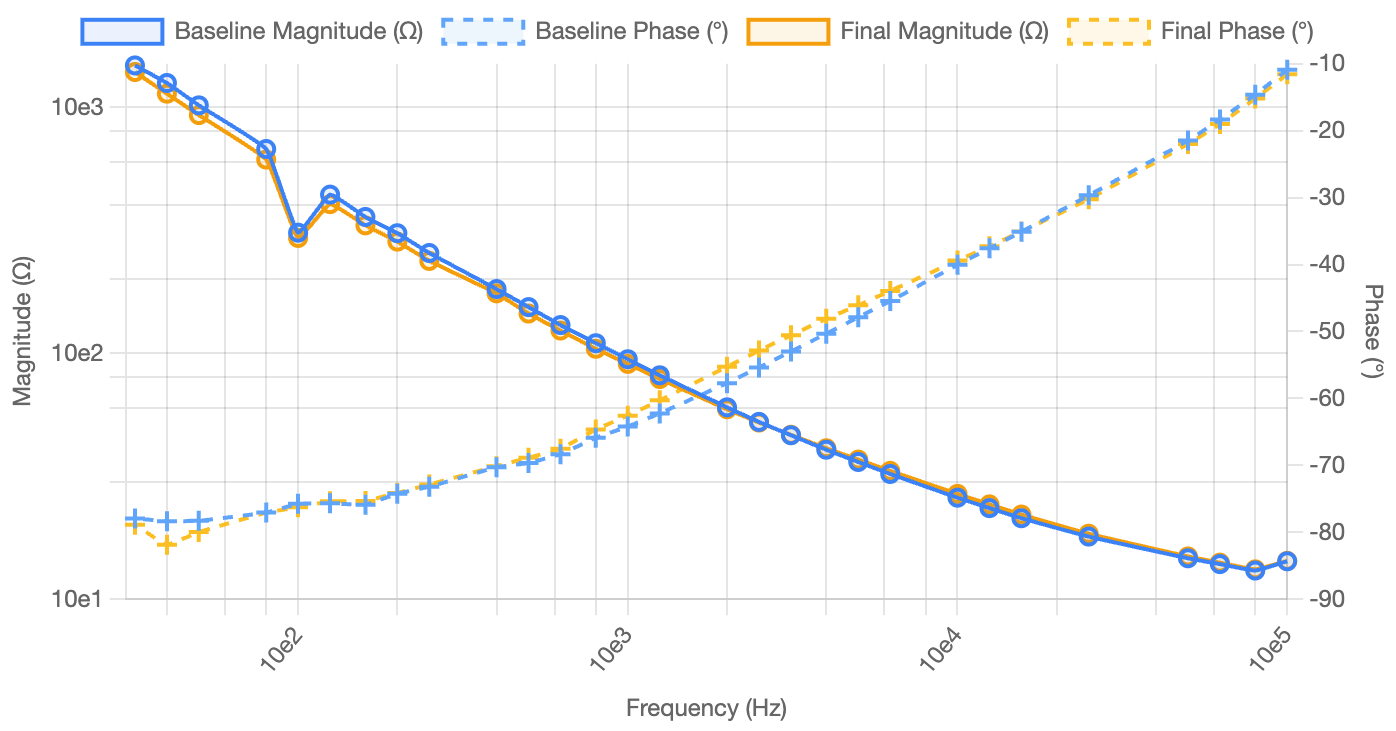
\includegraphics[width=\textwidth]{2g-100mL BioPal.png}
        \caption{BioPal: Baseline vs Post-BSA}
        \label{fig:2g_biopal}
    \end{subfigure}
    \hfill
    \begin{subfigure}{0.48\textwidth}
        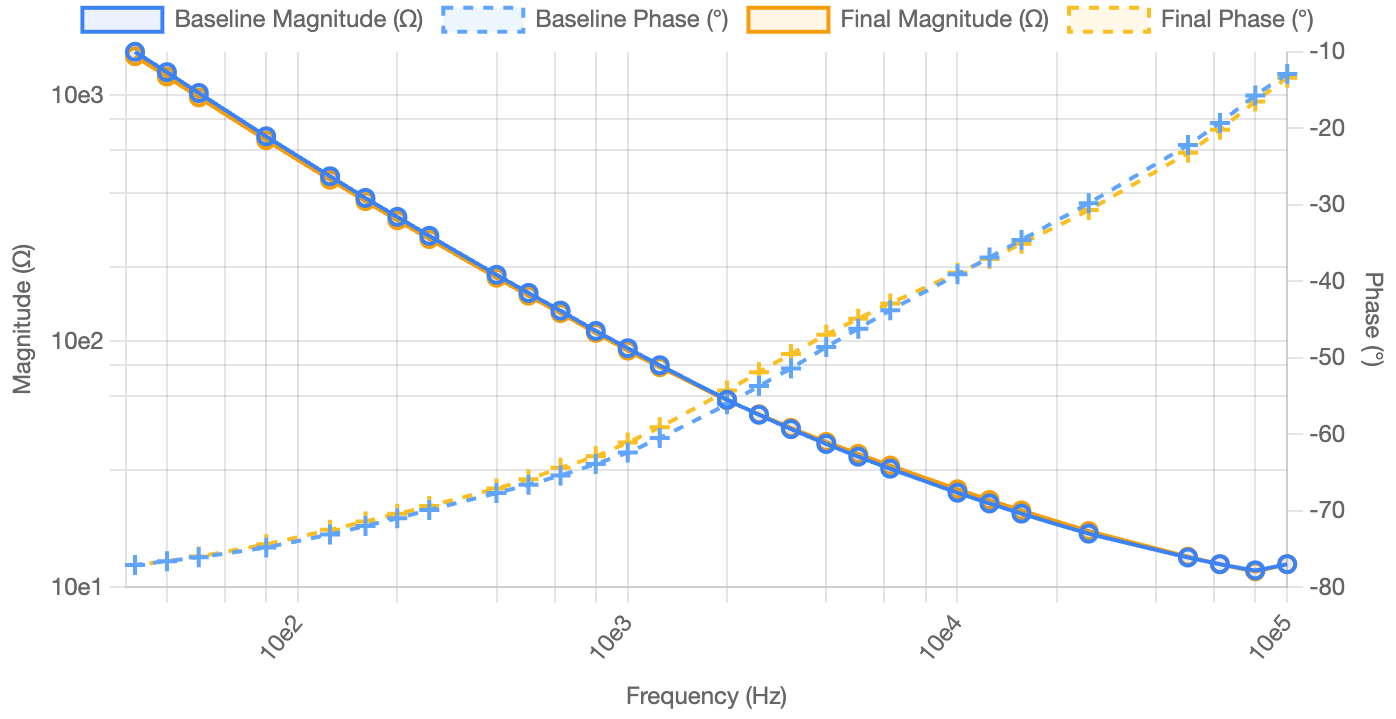
\includegraphics[width=\textwidth]{PalmSens2g.png}
        \caption{PalmSens4: Baseline vs Post-BSA}
        \label{fig:2g_palmsens}
    \end{subfigure}
    \caption{Baseline vs Final Frequency Response to 20mg/mL BSA Binding}
    \label{fig:2g_bsa_comparison_final}
\end{figure}

\begin{figure}[H]
    \centering
    \begin{subfigure}{0.48\textwidth}   
        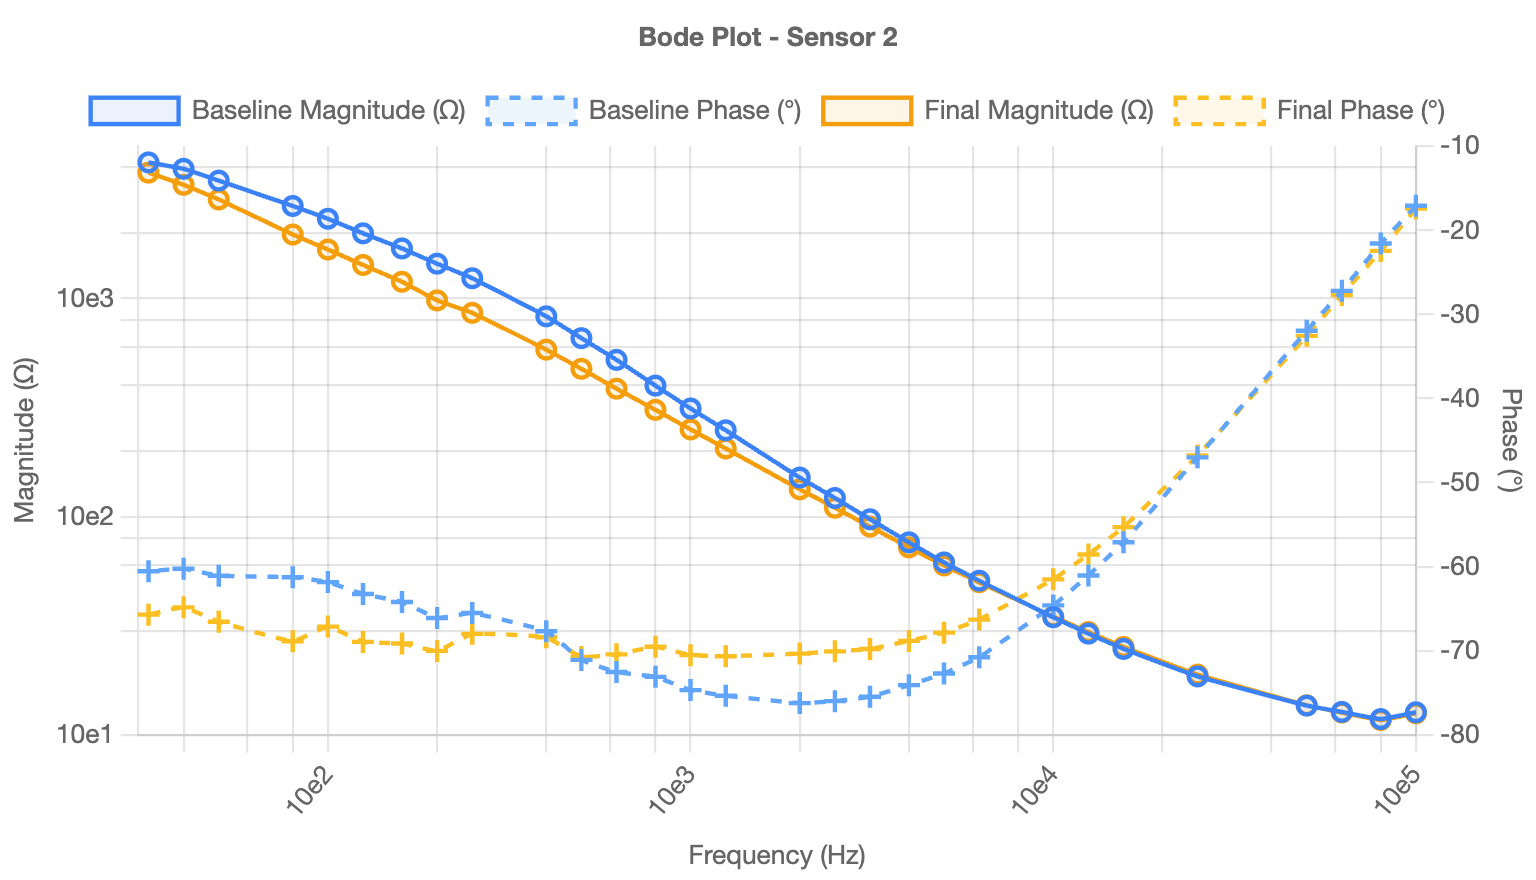
\includegraphics[width=\textwidth]{5g-100mL BioPal.png}
        \caption{BioPal: Baseline vs Post-BSA}
        \label{fig:5g_biopal}
    \end{subfigure}
    \hfill
    \begin{subfigure}{0.48\textwidth}
        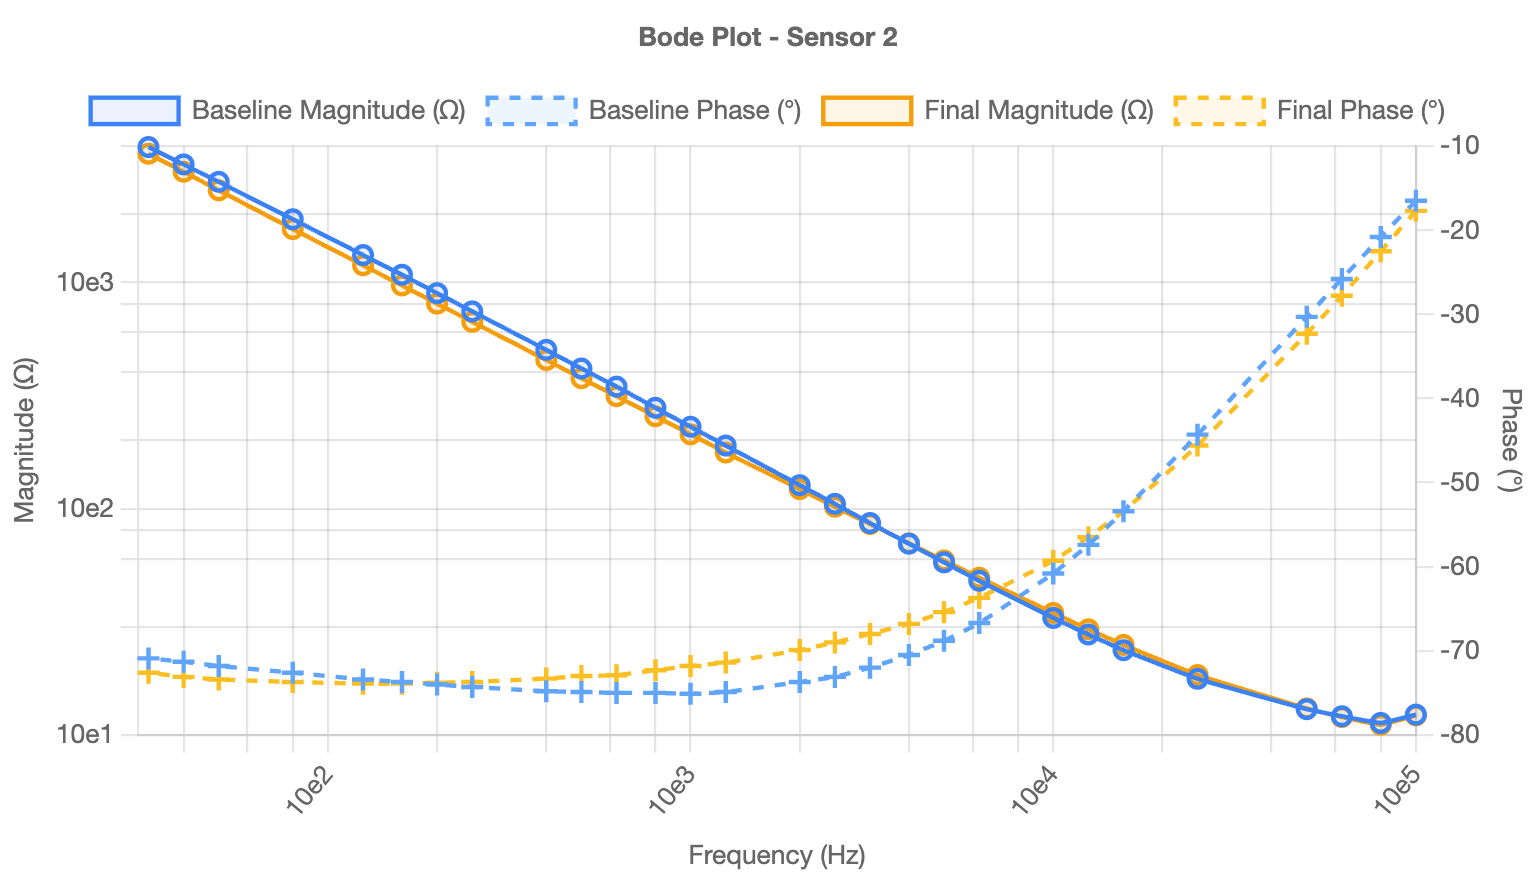
\includegraphics[width=\textwidth]{PalmSens5g.png}
        \caption{PalmSens4: Baseline vs Post-BSA}
        \label{fig:5g_palmsens}
    \end{subfigure}
    \caption{Baseline vs Final Frequency Response to 50mg/mL BSA Binding}
    \label{fig:5g_bsa_comparison_final}
\end{figure}

\begin{figure}[H]
    \centering
    \begin{subfigure}{0.48\textwidth}
        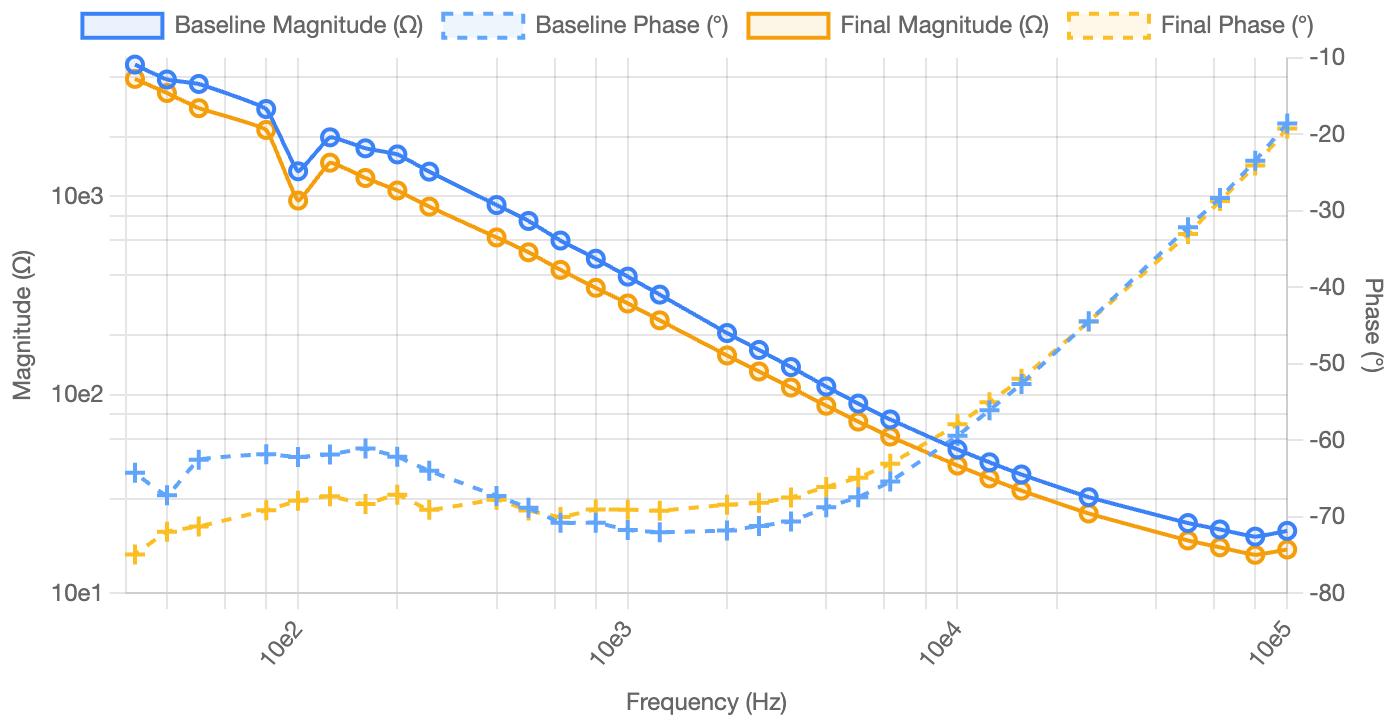
\includegraphics[width=\textwidth]{10g-100mL BioPal.png}   
        \caption{BioPal: Baseline vs Post-BSA}
        \label{fig:10g_biopal}
    \end{subfigure}
    \hfill
    \begin{subfigure}{0.48\textwidth}
        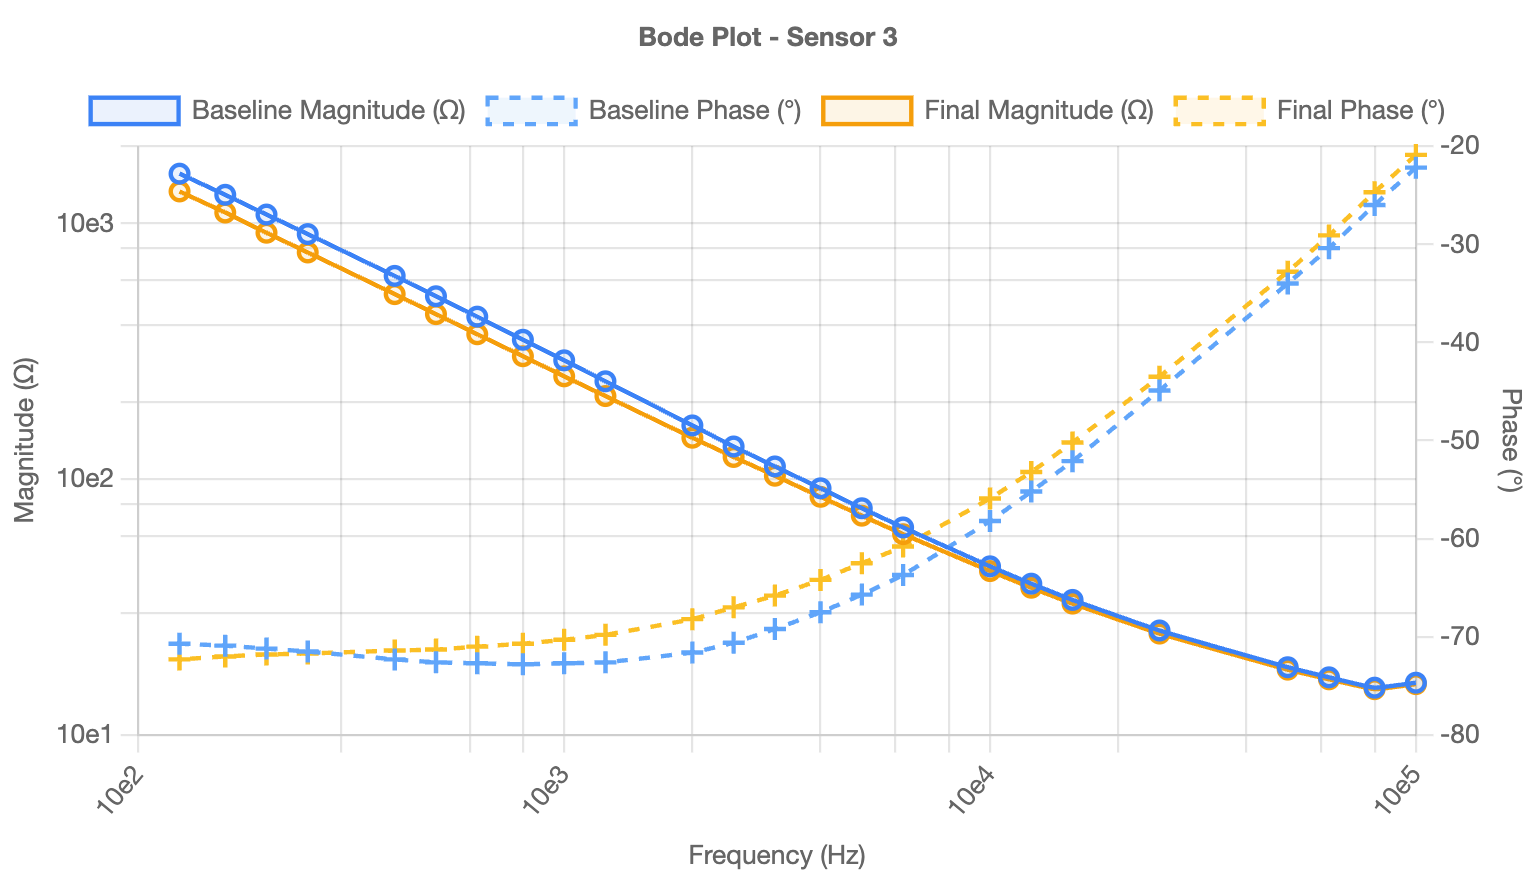
\includegraphics[width=\textwidth]{PalmSens10g.png}
        \caption{PalmSens4: Baseline vs Post-BSA}
        \label{fig:10g_palmsens}
    \end{subfigure}
    \caption{Baseline vs Final Frequency Response to 100mg/mL BSA Binding}
    \label{fig:10g_bsa_comparison_final}
\end{figure}

% 3 seperate figures with subfigures (not minipages) showing the change in magnitude and phase for both instruments
\begin{figure}[H]
    \centering
    \begin{subfigure}{0.48\textwidth}
        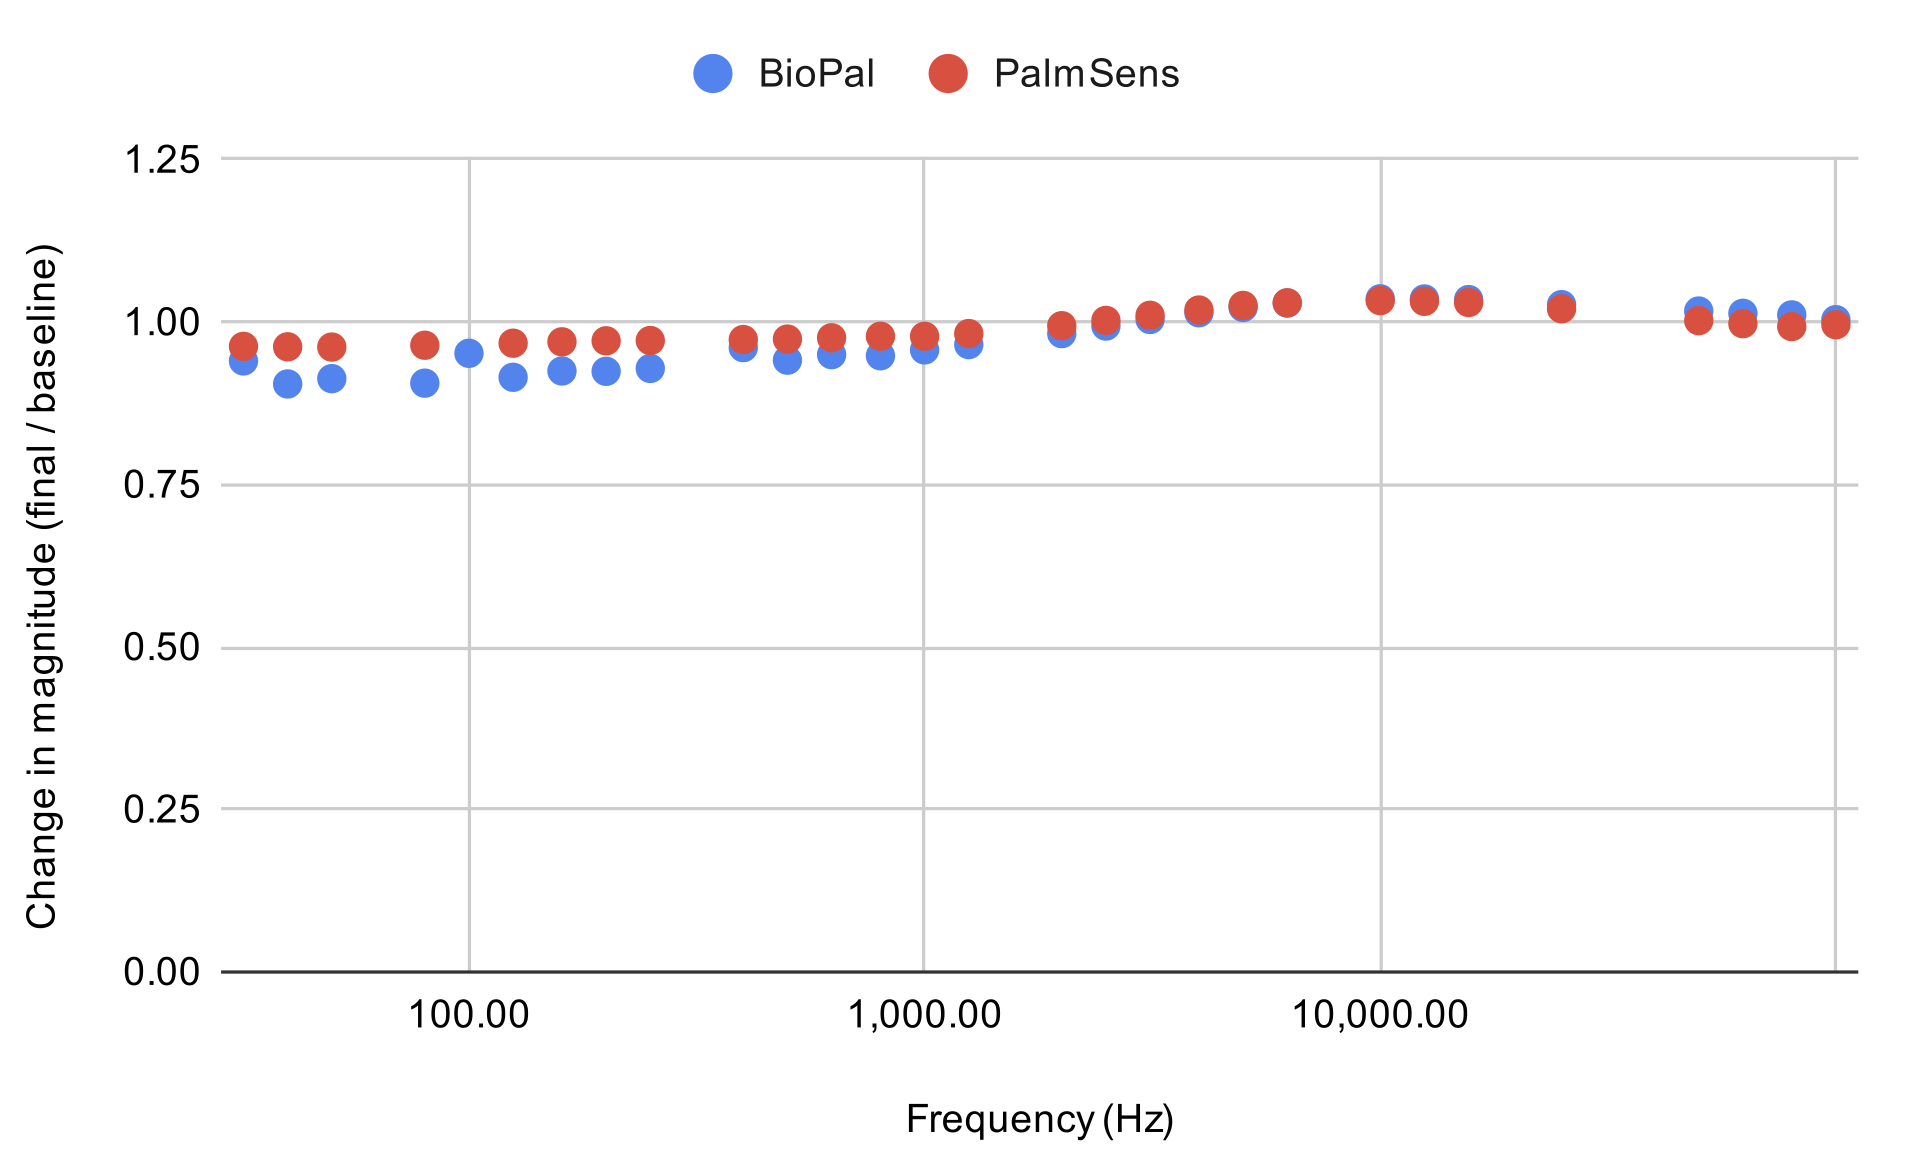
\includegraphics[width=\textwidth]{2g:100mL mag.png}
        \caption{Change in Impedance Magnitude}
        \label{fig:2g_mag}
    \end{subfigure}
    \hfill
    \begin{subfigure}{0.48\textwidth}
        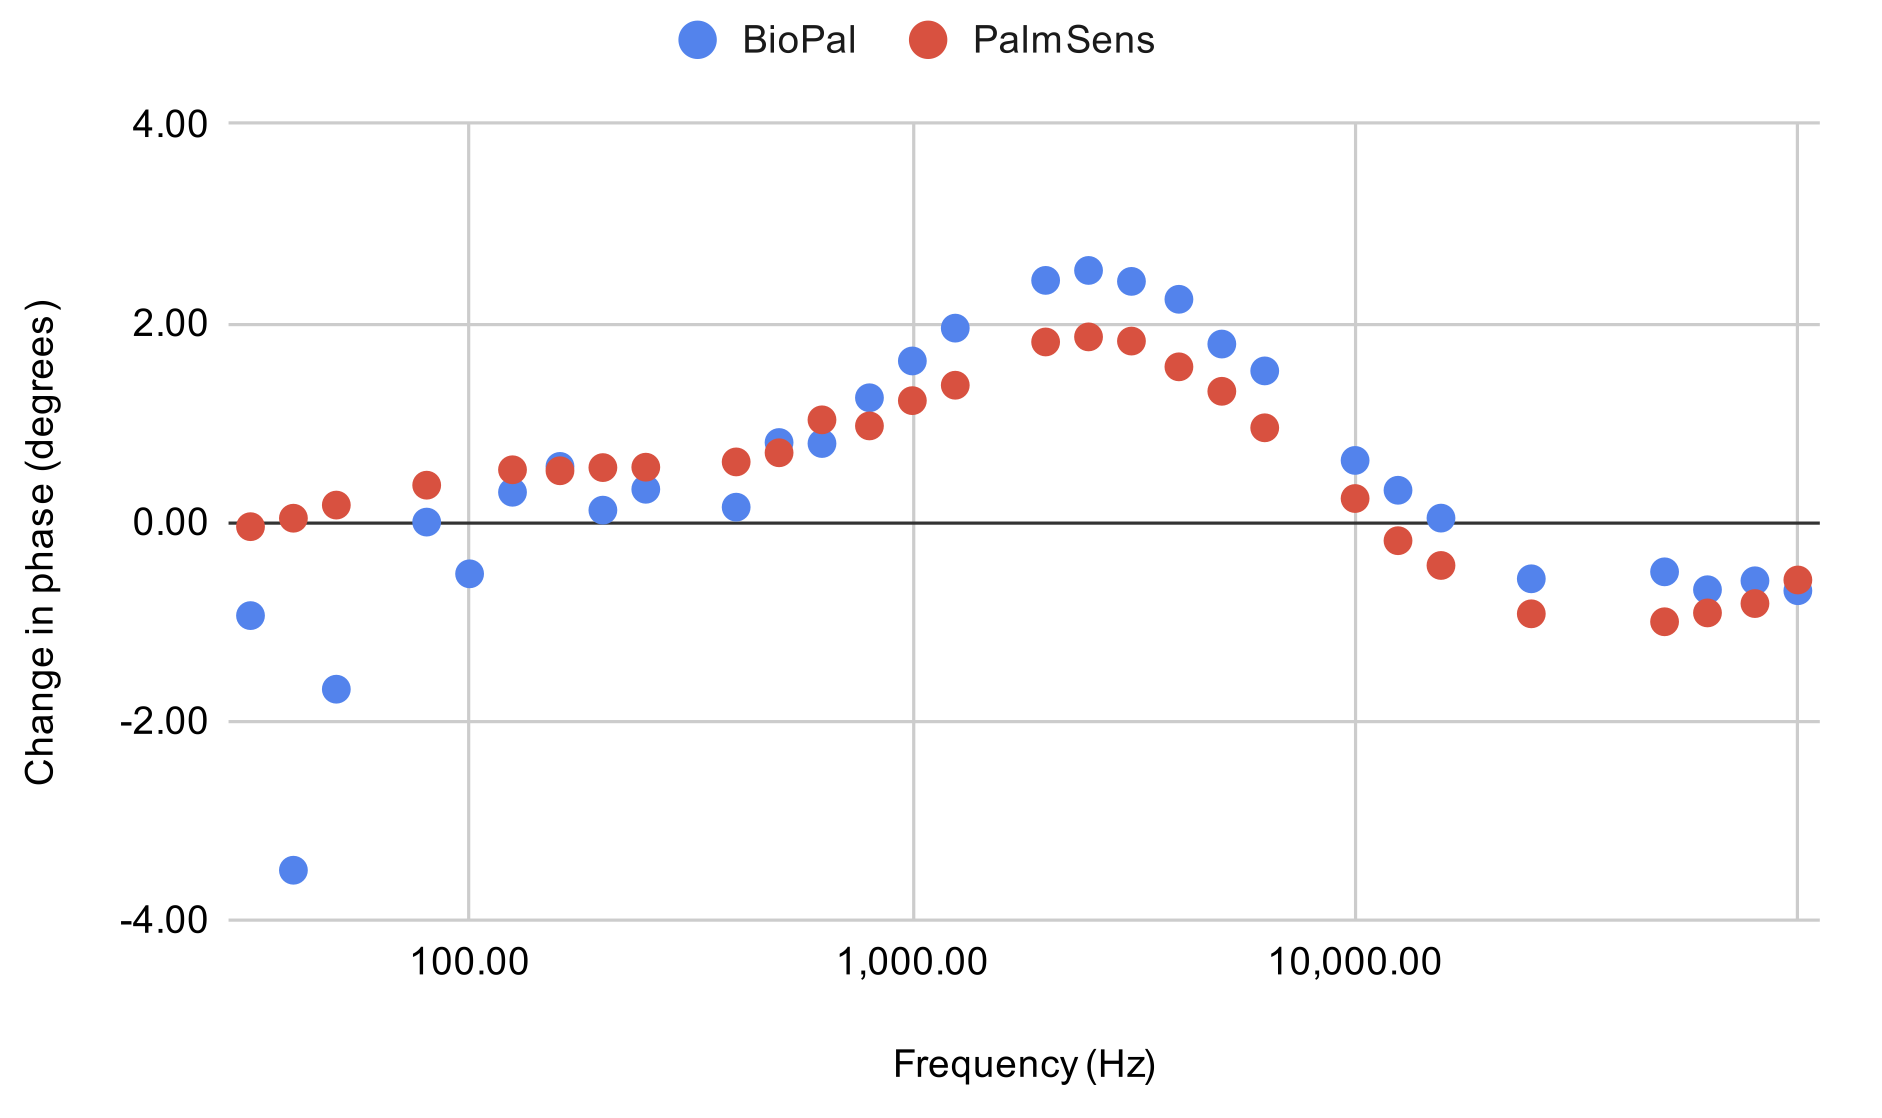
\includegraphics[width=\textwidth]{2g:100mL phase.png}
        \caption{Change in Impedance Phase}
        \label{fig:2g_phase}
    \end{subfigure}
    \caption{IDE Impedance Change with 2g/100mL BSA Binding}
    \label{fig:2g_bsa_comparison}
\end{figure}

% 5g/100mL BSA
\begin{figure}[H]
    \centering
    \begin{subfigure}{0.48\textwidth}   
        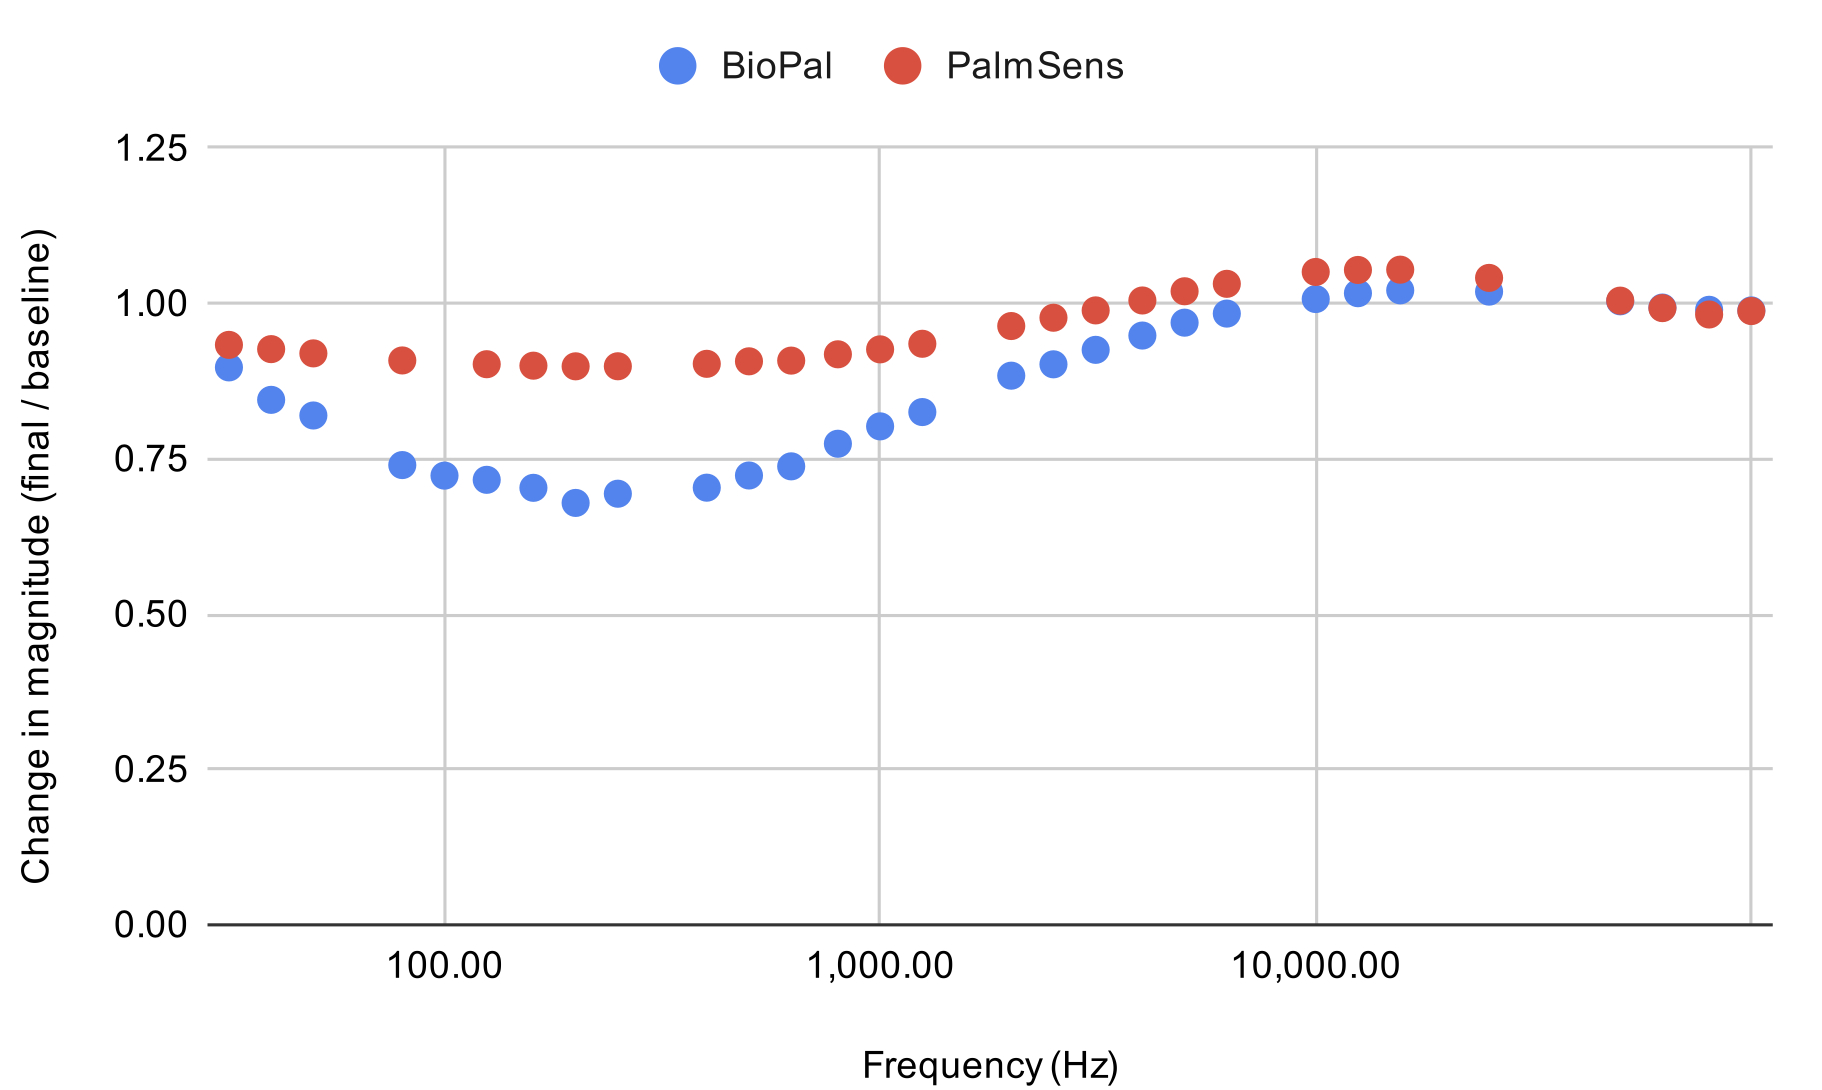
\includegraphics[width=\textwidth]{5g:100mL mag.png}
        \caption{Change in Impedance Magnitude}
        \label{fig:5g_mag}
    \end{subfigure}
    \hfill
    \begin{subfigure}{0.48\textwidth}
        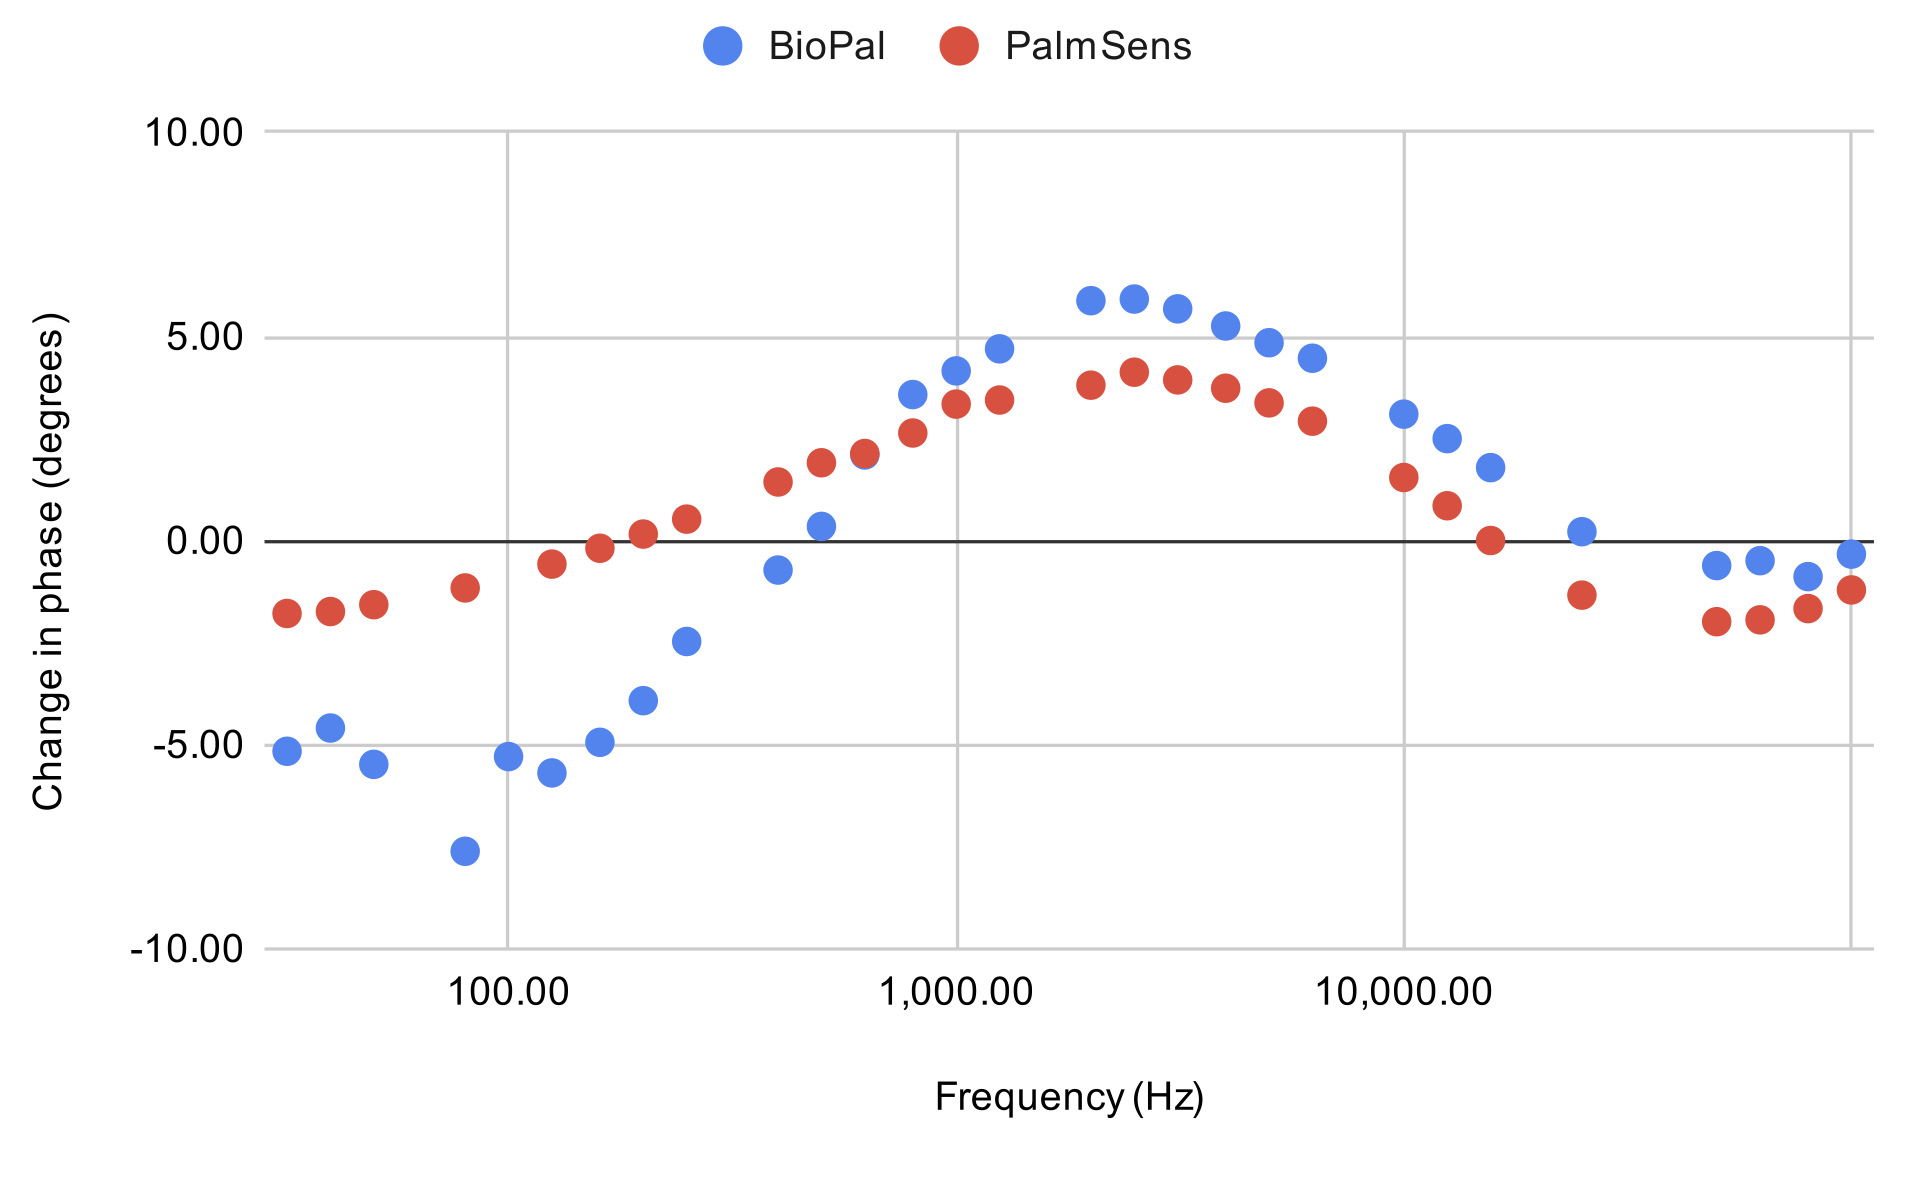
\includegraphics[width=\textwidth]{5g:100mL phase.png}
        \caption{Change in Impedance Phase}
        \label{fig:5g_phase}
    \end{subfigure}
    \caption{IDE Impedance Change with 5g/100mL BSA Binding}
    \label{fig:5g_bsa_comparison}
\end{figure}

% 10g/100mL BSA
\begin{figure}[H]
    \centering
    \begin{subfigure}{0.48\textwidth}
        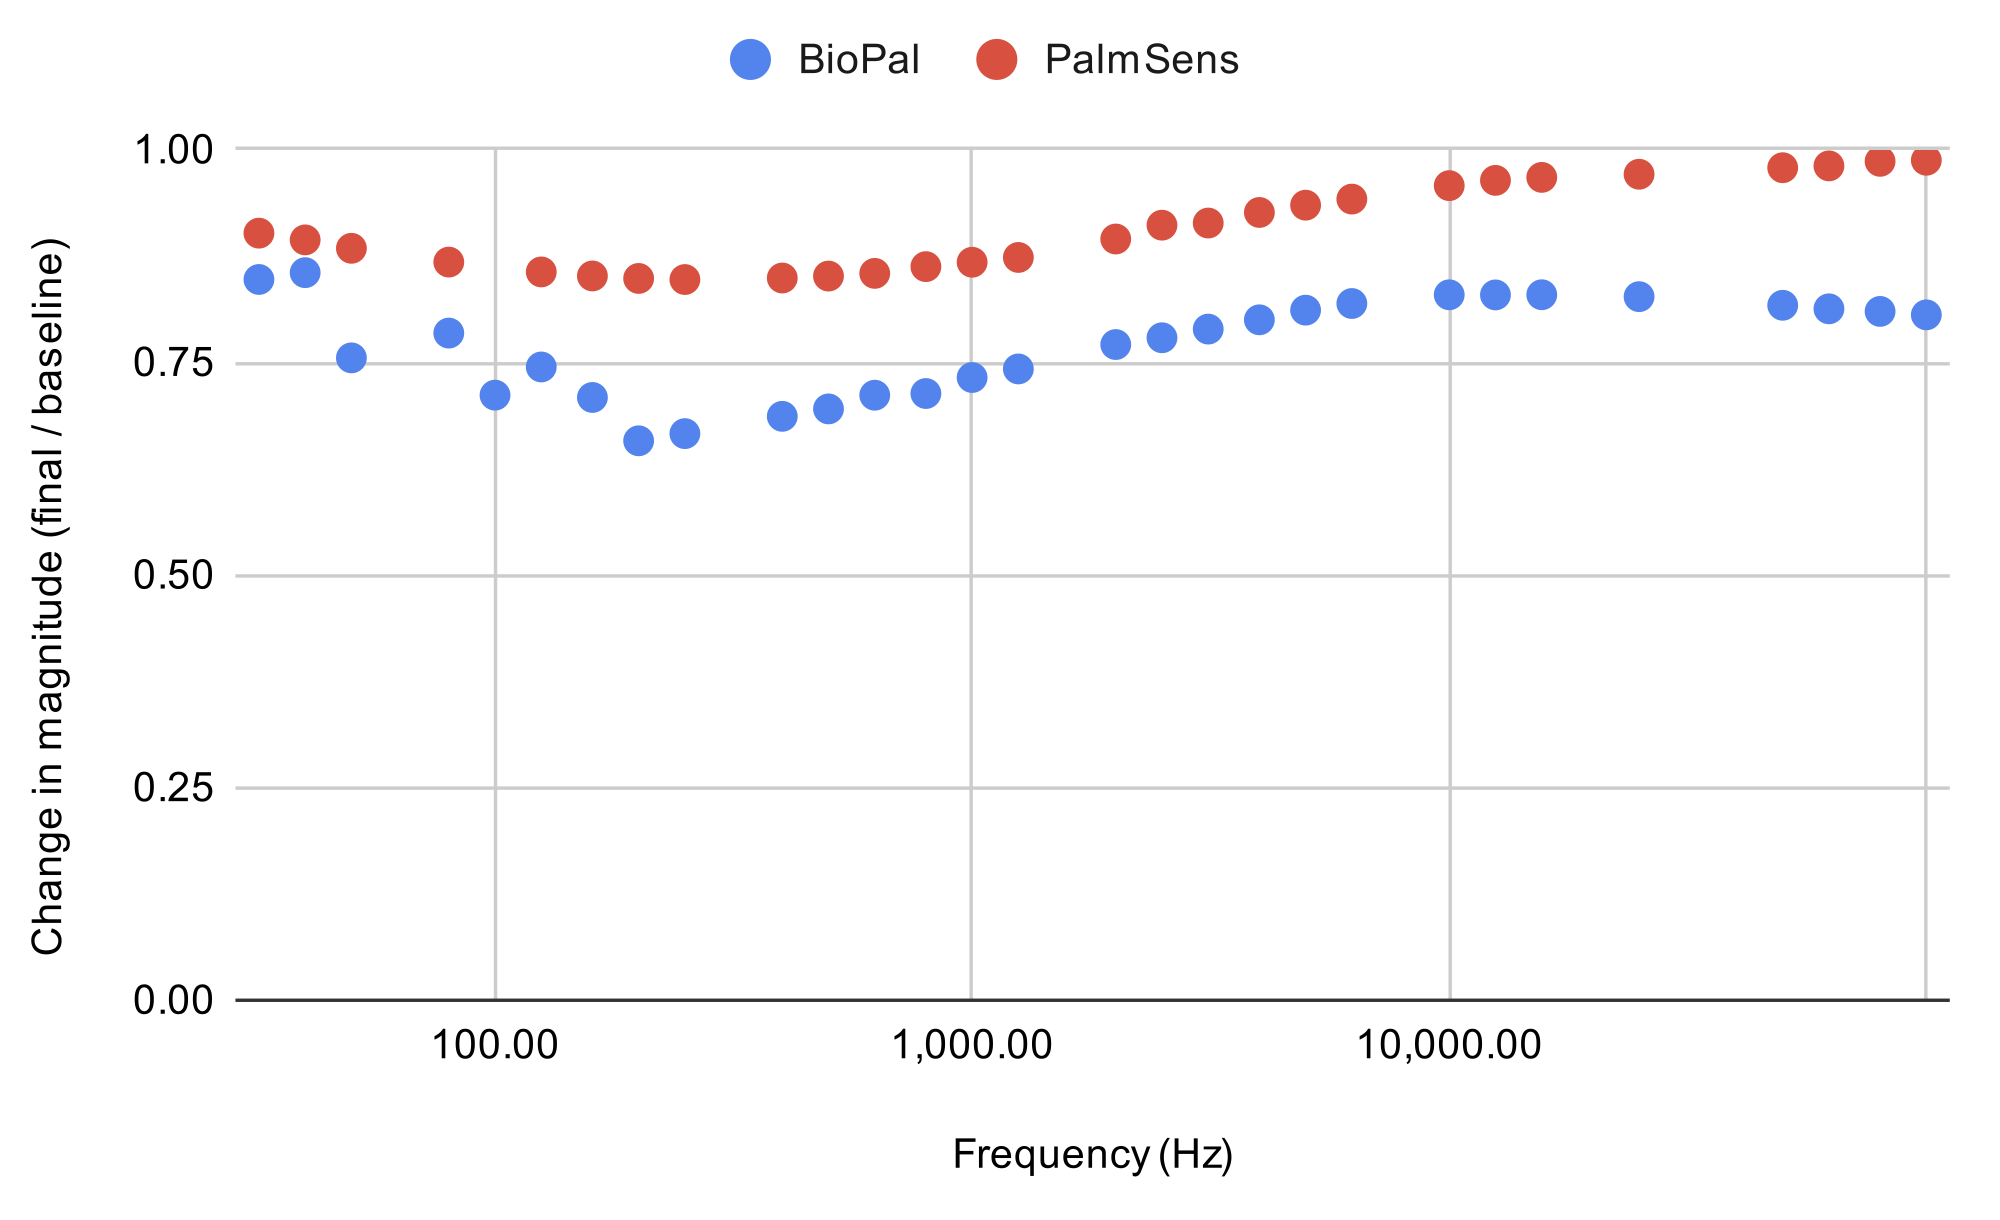
\includegraphics[width=\textwidth]{10g:100mL mag.png}   
        \caption{Change in Impedance Magnitude}
        \label{fig:10g_mag}
    \end{subfigure}
    \hfill
    \begin{subfigure}{0.48\textwidth}
        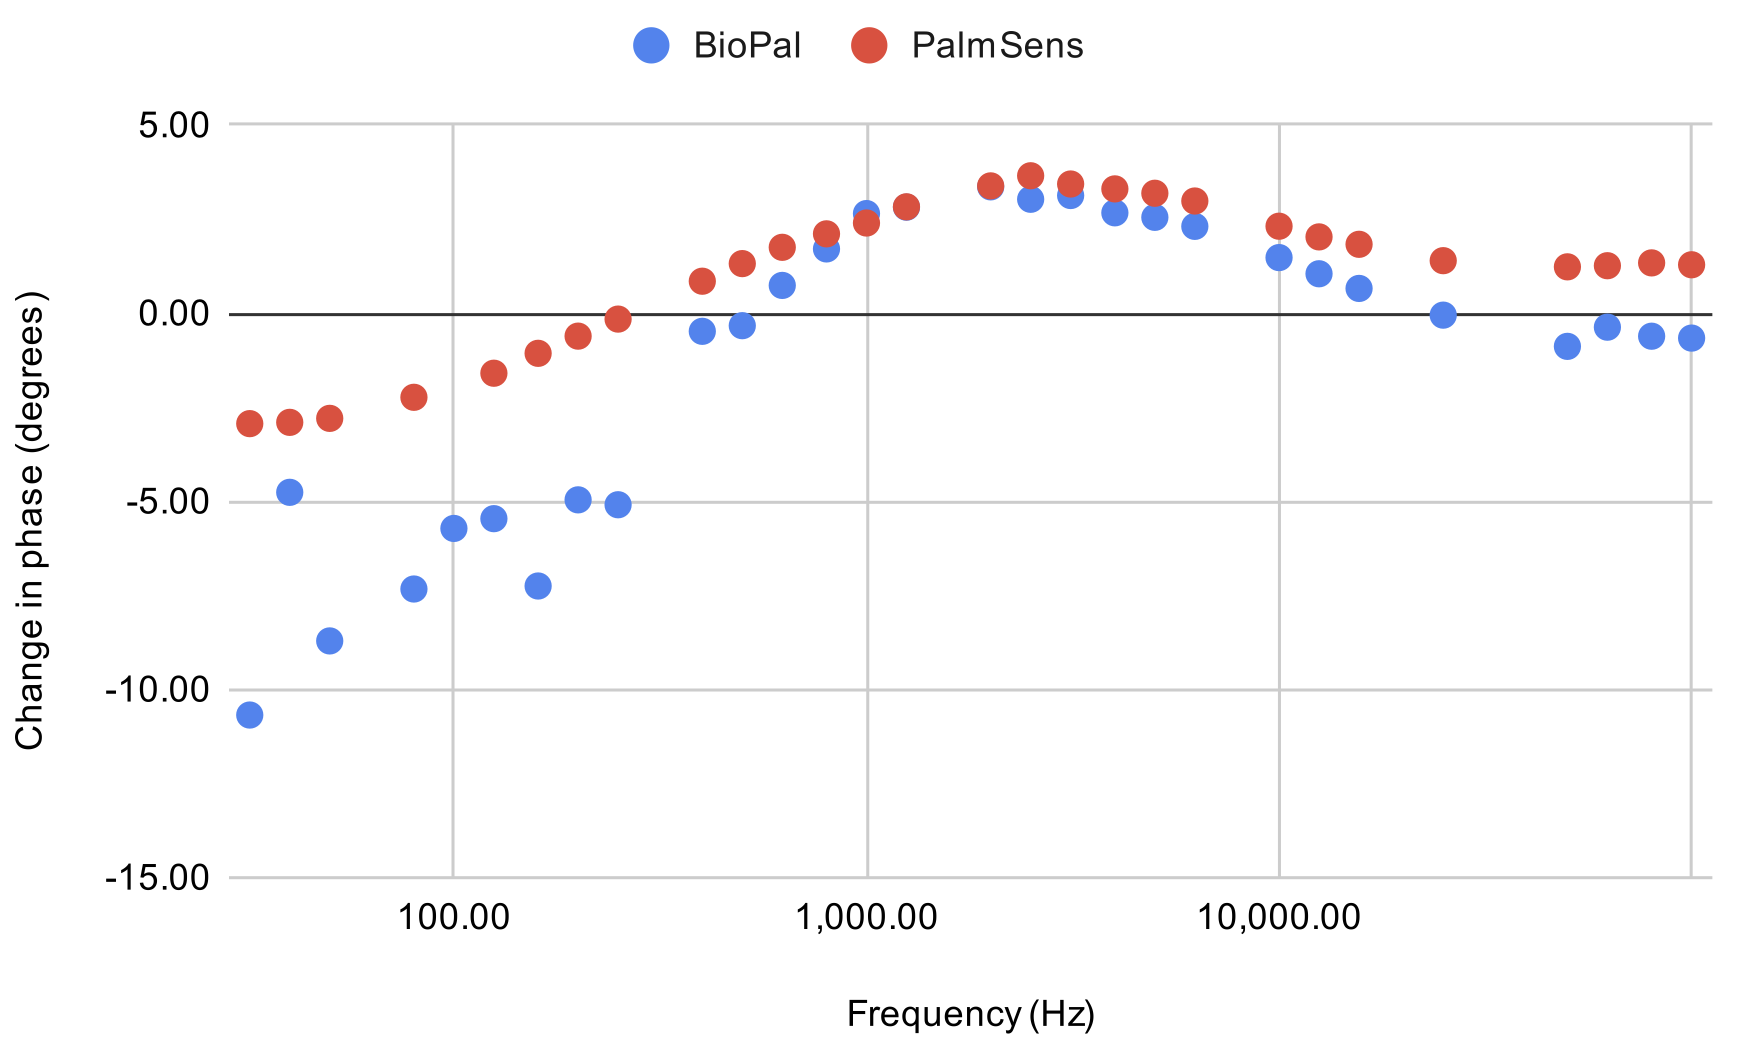
\includegraphics[width=\textwidth]{10g:100mL phase.png}
        \caption{Change in Impedance Phase}
        \label{fig:10g_phase}
    \end{subfigure}
    \caption{IDE Impedance Change with 10g/100mL BSA Binding}
    \label{fig:10g_bsa_comparison}
\end{figure}

\section{Discussion of Validation Results}

% The BioPal's performance varied across the measurement frequency range, with distinct regions of accuracy. At very low frequencies (below \todo{X Hz}), the biosensor impedance becomes extremely high, resulting in currents in the tens of nanoamperes. At these current levels, the signal-to-noise ratio decreases substantially, making it difficult to distinguish the frequency content of interest from background noise. Consequently, measurements in this region exhibited large error margins. However, the overall trend still aligned with PalmSens4 measurements, indicating that whilst absolute accuracy was compromised, the relative changes were correctly captured.

% At slightly higher frequencies (\todo{X Hz to X Hz}), measurement accuracy improved dramatically as current levels increased and the signal-to-noise ratio became more favourable. Error margins reduced substantially, though some discrepancy from the PalmSens4 remained visible. The optimal measurement range was found to be \todo{X Hz to X Hz}, where error margins were minimal and measurements closely tracked the reference instrument. This frequency range aligns well with the region where surface characteristic changes are most prominent in EIS biosensing, making it particularly relevant for detecting analyte binding events. These are the frequencies where changes in the double-layer capacitance and charge transfer resistance due to biomolecular interactions at the electrode surface are most readily observable.

% At very high frequencies (above \todo{X Hz}), error margins increased slightly again. This can be attributed to several factors: the phase shifts in the measurement circuitry become more significant, the absence of the anti-aliasing filter allows more high-frequency noise into the system, and the parasitic capacitances and inductances in the PCB layout begin to affect measurements more noticeably.

% Despite these frequency-dependent variations in accuracy, the BioPal successfully demonstrated its core capability: detecting and quantifying impedance changes at key frequencies relevant to biosensing. The device clearly distinguished between baseline and post-BSA measurements, identifying the characteristic impedance increase associated with protein binding to the electrode surface. This validates the BioPal's applicability for quantitative biosensor measurements in point-of-care settings.

% The results demonstrate that the BioPal can provide point-of-care healthcare professionals with a low-cost, portable tool for rapid disease screening. Whilst it does not match the precision of laboratory-grade instruments like the PalmSens4 across the entire frequency spectrum, it performs well in the critical frequency ranges for biosensor applications. This enables healthcare workers to quickly screen patients and identify individuals who require further testing or specialist referral, without the need for expensive laboratory equipment or extensive technical training. The device thus fulfils its design objective of democratising biosensor-based diagnostics for resource-limited settings.

\newpage
\newpage
\label{chap:testing_and_validation}